\documentclass[12pt]{article}
\usepackage[utf8]{inputenc}
\usepackage[english]{babel}
\usepackage{amsmath, amssymb, amsthm, bm}
\usepackage{geometry}
\usepackage{tikz}
\usetikzlibrary{shapes, backgrounds, positioning, arrows.meta, calc, decorations.pathreplacing}
\usepackage{caption}
\usepackage{setspace}
\usepackage{enumitem}
\usepackage{booktabs}
\usepackage[authordate,backend=biber,style=chicago-authordate]{biblatex}

% Bibliography file link
\addbibresource{references.bib}

\geometry{letterpaper, margin=1in}
\onehalfspacing

% Custom theorem styles
\newtheorem{theorem}{Theorem}[section]
\newtheorem{definition}{Definition}[section]
\newtheorem{example}{Example}[section]

\begin{document}

\title{\textbf{Formal Mathematical Definition and Equivalence Proof: \\ 
The Tool Switching Problem and the Generalized Traveling Salesman Problem}}
\author{Shankar Narayanan \\ \textit{Internship Report} \\ \textit{Advisor: Prof. Annegret Wagler}}
\date{March 30, 2026}

\maketitle

\begin{abstract}
This report provides a rigorous mathematical analysis of the Standard Tool Switching Problem (SSP) in automated manufacturing. We formally define the problem parameters using the framework of \textcite{Colares2026}, presenting their non-compact integer programming formulation. A primary objective is to demonstrate the mathematical equivalence between the SSP and the Generalized Traveling Salesman Problem (GTSP) through vertex duplication and distance-preserving mapping. Furthermore, we explore the integration of Machine Learning (ML) within a Column Generation framework to address the exponential state space.
\end{abstract}

\newpage

\section{Introduction}
In modern flexible manufacturing systems (FMS) and Computer Numerical Control (CNC) machining, tool management is a critical bottleneck[cite: 146]. The Tool Switching Problem (SSP) addresses the challenge of sequencing jobs on a machine with a tool magazine of limited capacity $B$[cite: 147]. Every job requires a specific subset of tools; if the required tools are not currently loaded, a "switch" must occur, incurring setup costs in terms of time and mechanical wear[cite: 148]. 

Historically, this problem has been categorized as NP-hard, necessitating exact combinatorial models as production schedules grow in complexity[cite: 150]. This report bridges the gap between the SSP and the Generalized Traveling Salesman Problem (GTSP) to leverage advanced solvers and neural-augmented techniques[cite: 151].

\section{The Baseline Heuristic: KTNS}
Before defining exact models, it is essential to understand the "Keep Tool Needed Soonest" (KTNS) rule, the standard greedy baseline for tool management. 

\begin{definition}[KTNS Rule]
Given a fixed sequence of jobs, if a tool must be removed to make room for a required tool, the tool whose next required execution is furthest in the future should be ejected from the magazine.
\end{definition}

While KTNS is optimal for a \textit{fixed} job sequence, the SSP seeks the optimal \textit{permutation} of jobs, making the problem significantly more complex as the sequence itself becomes a decision variable.

\section{Formal Definition of the Tool Switching Problem (SSP)}

Following the formalisms of \textcite{Colares2026}, the SSP is defined as follows:

\subsection{Sets and Parameters}
\begin{itemize}
    \item \textbf{The Job Set:} $J = \{j_1, j_2, \dots, j_n\}$ represents the set of tasks to be completed[cite: 152].
    \item \textbf{The Tool Set:} $T = \{t_1, t_2, \dots, t_m\}$ contains all unique tools available[cite: 153].
    \item \textbf{Requirements:} Each job $j_i \in J$ requires a subset $T_i \subseteq T$[cite: 154].
    \item \textbf{Capacity:} The magazine has capacity $B$[cite: 155]. A configuration $C \subseteq T$ is valid if $|C| \le B$[cite: 156].
\end{itemize}

\subsection{Operational Feasibility and Switching}
A job $j_i$ is feasible if $T_i \subseteq C_{current}$. If $T_i \not\subseteq C_{current}$, a switching operation replaces an unnecessary tool $t_{out} \in C \setminus T_i$ with $t_{in} \in T_i \setminus C$ [cite: 159-160]. The objective is to find a permutation $\sigma$ of $J$ that minimizes total switches $Z$[cite: 161].

\section{Illustrative Example: Magazine State Evolution}
To illustrate the switching mechanics, consider an instance with $B=3$ and $J=\{j_1, j_2, j_3\}$:
\begin{itemize}
    \item $T_1 = \{t_1, t_2\}$, $T_2 = \{t_2, t_3\}$, $T_3 = \{t_1, t_3, t_4\}$ (Note: $|T_3|=3=B$).
\end{itemize}

\begin{figure}[h!]
\centering
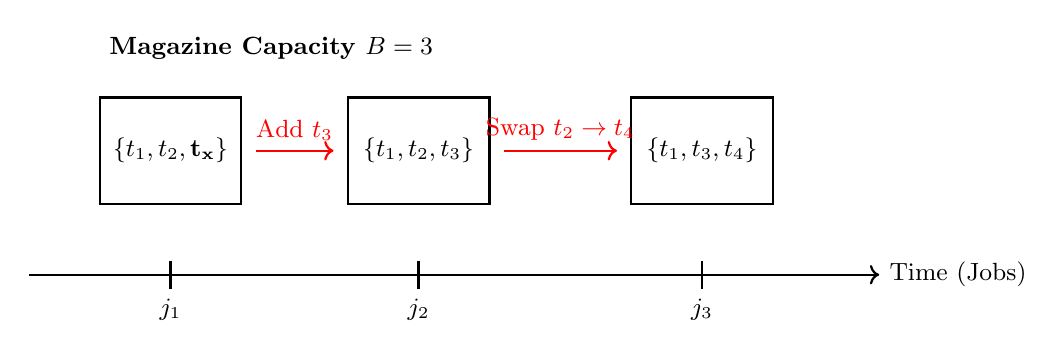
\begin{tikzpicture}[scale=0.9, every node/.style={font=\small}]
    % Time Axis
    \draw[->, thick] (-1,0) -- (11,0) node[right] {Time (Jobs)};
    
    % Job Markers
    \foreach \x/\t in {1/j_1, 4.5/j_2, 8.5/j_3} {
        \draw[thick] (\x, 0.2) -- (\x, -0.2) node[below] {$\t$};
    }

    % Magazine Slots
    \draw[thick] (0,1) rectangle (2,2.5) node[midway] {$\{t_1, t_2, \mathbf{t_x}\}$};
    \draw[thick] (3.5,1) rectangle (5.5,2.5) node[midway] {$\{t_1, t_2, t_3\}$};
    \draw[thick] (7.5,1) rectangle (9.5,2.5) node[midway] {$\{t_1, t_3, t_4\}$};

    % Switch Indicators
    \draw[->, red, thick] (2.2, 1.75) -- (3.3, 1.75) node[midway, above] {Add $t_3$};
    \draw[->, red, thick] (5.7, 1.75) -- (7.3, 1.75) node[midway, above] {Swap $t_2 \to t_4$};

    \node[anchor=west] at (0,3.2) {\textbf{Magazine Capacity $B=3$}};
\end{tikzpicture}
\caption{State-space timeline of a tool magazine. Transitions between jobs $j_2$ and $j_3$ require a tool swap because $T_3$ consumes the entire capacity $B$.}
\label{fig:magazine_timeline}
\end{figure}

\section{The Colares-Wagler Non-Compact Formulation}

The complexity of the SSP is fundamentally rooted in the size of the state space. As the number of configurations $p = \binom{m}{B}$ is exponential, traditional compact models for the TSP cannot be directly applied without a decomposition strategy . \textcite{Colares2026} propose a non-compact formulation that models the problem as a set-covering task integrated with a sequencing task on a graph of configurations.

\subsection{Decision Variables}
Let $V$ be the vertex set representing the collection of all possible tool repository configurations $\mathcal{C}$ [cite: 28-29]. The model utilizes two primary sets of binary decision variables :
\begin{itemize}
    \item $y(v) \in \{0, 1\}$: Equals 1 if configuration $v \in V$ is selected to process at least one job, 0 otherwise.
    \item $x(u, v) \in \{0, 1\}$: Equals 1 if the machine transitions from configuration $u$ to configuration $v$.
\end{itemize}

\subsection{Mathematical Model}
The objective is to minimize the total tool switching operations across the entire sequence[cite: 55]:
\begin{equation}
    \min Z = \sum_{u \in V} \sum_{v \in V} d(u, v) x(u, v)
\end{equation}

Subject to the following structural constraints [cite: 56-75]:
\begin{align}
    \sum_{v \in H_j} y(v) \geq 1 & \quad \forall j \in J \label{eq:cover_cons} \\
    \sum_{u \in V} x(u, v) = y(v) & \quad \forall v \in V \label{eq:flow_in_cons} \\
    \sum_{u \in V} x(v, u) = y(v) & \quad \forall v \in V \label{eq:flow_out_cons} \\
    \sum_{u \in H(S)} \sum_{v \in H(S)} x(u, v) \leq \sum_{v \in H(S)} y(v) - 1 & \quad \forall S \subseteq J, 2 \leq |S| \leq |J|-1 \label{eq:sec_cons}
\end{align}

Where $H_j = \{C_i \in \mathcal{C} : T_j \subseteq C_i\}$ is the cluster of valid configurations for job $j$[cite: 34]. Constraint \eqref{eq:cover_cons} ensures that every job is associated with at least one used configuration. Constraints \eqref{eq:flow_in_cons} and \eqref{eq:flow_out_cons} enforce that selected configurations are connected in a continuous path. Equation \eqref{eq:sec_cons} represents the Subtour Elimination Constraints (SEC) applied over the union of job clusters $H(S) = \bigcup_{j \in S} H_j$ [cite: 67-68, 75].

\section{Metric Properties of the Configuration Space}

The distance function $d(u,v)$ is not merely an arbitrary cost but a rigorous metric that defines the geometry of the configuration graph $K_p$.

\subsection{Formal Definition of Distance}
For any two configurations $C_i$ and $C_j$, the distance is calculated based on the symmetric difference of their toolsets, specifically focusing on the number of tools that must be added (which, in a full magazine, equals the number of tools removed) [cite: 31-32]:
\begin{equation}
    d(i, j) = B - |C_i \cap C_j|
\end{equation}

\subsection{Triangular Inequality Proof}
\begin{lemma}[Triangular Inequality]
For any three vertices $u, w, v \in V$, the inequality $d(u, v) \le d(u, w) + d(w, v)$ holds .
\end{lemma}
\begin{proof}
Let $|C_u \cap C_v|$ be the number of tools shared between configurations $u$ and $v$. The distance $d(u,v)$ is proportional to the size of the set $C_u \setminus C_v$. Since set differences in a finite universe satisfy the triangle inequality under the cardinality operator, it follows that the number of swaps to move from $u$ to $v$ via an intermediate state $w$ is at least as large as the direct swap .
\end{proof}

\section{Hypergraph Representation of Job Overlaps}

The "Overlap Problem" can be visualized as a hypergraph $\mathcal{H} = (T, \mathcal{J})$, where tools are nodes and each job $j \in J$ is a hyper-edge connecting the tools it requires. When two hyper-edges share nodes, their corresponding configuration clusters $H_j$ in $K_p$ will overlap.

\begin{figure}[h!]
\centering
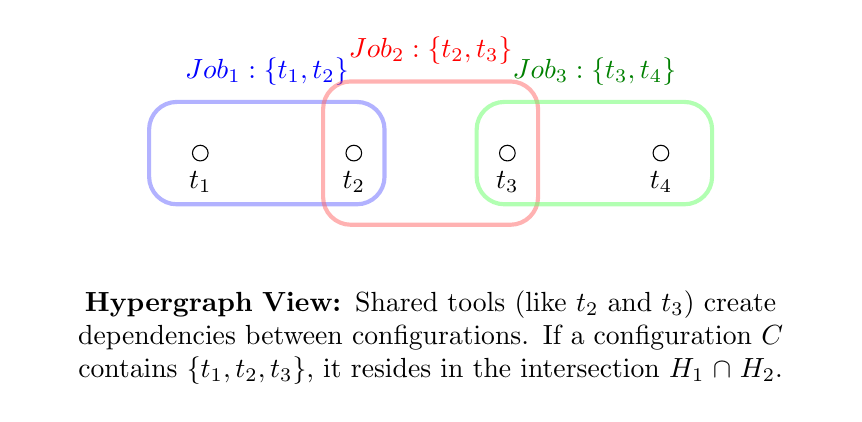
\begin{tikzpicture}[scale=1.3]
    % Tools as base nodes
    \node[draw, circle, inner sep=2pt, label=below:{$t_1$}] (t1) at (0,0) {};
    \node[draw, circle, inner sep=2pt, label=below:{$t_2$}] (t2) at (1.5,0) {};
    \node[draw, circle, inner sep=2pt, label=below:{$t_3$}] (t3) at (3,0) {};
    \node[draw, circle, inner sep=2pt, label=below:{$t_4$}] (t4) at (4.5,0) {};

    % Job 1 as a Hyperedge
    \draw[line width=1.5pt, blue!60, opacity=0.5, rounded corners=10pt] 
        (-0.5,-0.5) rectangle (1.8, 0.5);
    \node[blue] at (0.65, 0.8) {$Job_1: \{t_1, t_2\}$};

    % Job 2 as a Hyperedge (overlapping at t2)
    \draw[line width=1.5pt, red!60, opacity=0.5, rounded corners=10pt] 
        (1.2,-0.7) rectangle (3.3, 0.7);
    \node[red] at (2.25, 1.0) {$Job_2: \{t_2, t_3\}$};

    % Job 3 (overlapping at t3, t4)
    \draw[line width=1.5pt, green!60, opacity=0.5, rounded corners=10pt] 
        (2.7,-0.5) rectangle (5.0, 0.5);
    \node[green!50!black] at (3.85, 0.8) {$Job_3: \{t_3, t_4\}$};

    \node[text width=10cm, align=center] at (2.25, -1.8) {
        \textbf{Hypergraph View:} Shared tools (like $t_2$ and $t_3$) create dependencies between configurations. If a configuration $C$ contains $\{t_1, t_2, t_3\}$, it resides in the intersection $H_1 \cap H_2$.
    };
\end{tikzpicture}
\caption{Hypergraph representation of tool requirements. Overlapping hyper-edges indicate jobs that can be "covered" by the same configuration nodes in the graph $K_p$.}
\label{fig:hypergraph}
\end{figure}

\section{The Overlap Problem in Tool Switching}

A fundamental mathematical distinction between the Standard Tool Switching Problem (SSP) and the classic Generalized Traveling Salesman Problem (GTSP) lies in the topology of the configuration clusters. In a standard GTSP, as defined in the survey by \textcite{Pop2024}, the vertex set is partitioned into \textbf{disjoint} sets $V_1, \dots, V_n$. Conversely, in the SSP, the combinatorial structure of tool requirements often dictates that a single configuration node $v \in V(K_p)$ satisfies the requirements of multiple jobs simultaneously .

\begin{definition}[Overlapping Clusters]
In an SSP instance, let $H_j$ be the cluster of configurations for job $j$. Two clusters $H_i$ and $H_k$ are overlapping if there exists at least one configuration $C$ such that $T_i \subseteq C$ and $T_k \subseteq C$. 
\end{definition}

This overlapping nature implies that the SSP is a composite of a \textbf{Covering Problem} (selecting configurations to satisfy job toolsets) and a \textbf{Traveling Salesman Problem} (sequencing those configurations) [cite: 36-39, 190]. To leverage exact GTSP solvers, this overlap must be mathematically linearized into disjoint partitions.

\section{Formal Reduction: $SSP \rightarrow GTSP$}

We demonstrate that any instance of the SSP can be reduced to a GTSP by expanding the state space through vertex duplication, a technique established in the literature by \textcite{Noon1993} and further refined by \textcite{Lien2015}.

\subsection{Mathematical Construction of the GTSP Graph}
Let $\mathcal{I}_{SSP} = (J, T, B, \{T_j\}_{j \in J})$ be an instance of the Tool Switching Problem. We construct a corresponding GTSP instance $\mathcal{I}_{GTSP} = (\mathcal{V}, \mathcal{E}, \{V_j\}_{j \in J})$ as follows:

\begin{enumerate}
    \item \textbf{Vertex Set Expansion:} For every configuration $C \in \mathcal{C}$ and every job $j \in J$ such that the configuration is capable of processing the job ($C \in H_j$), we define a unique GTSP vertex $v_{C,j}$ [cite: 34-35, 194].
    \item \textbf{Disjoint Partitioning:} We define the GTSP clusters as:
    \begin{equation}
        V_j = \{ v_{C,j} : C \in H_j \} \quad \forall j \in J
    \end{equation}
    By indexing each configuration node with its corresponding job identifier $j$, we ensure that $V_i \cap V_k = \emptyset$ for all $i \neq k$, regardless of whether the underlying configurations are identical[cite: 195].
    \item \textbf{Edge Weight Assignment:} The distance between two GTSP nodes $v_{C_u, i}$ and $v_{C_v, k}$ is inherited from the tool switching distance $d(u,v)$ defined in the configuration graph $K_p$:
    \begin{equation}
        w(v_{C_u, i}, v_{C_v, k}) = B - |C_u \cap C_v|
    \end{equation}
\end{enumerate}

\subsection{Proof of Equivalence}
\begin{theorem}
An optimal Hamiltonian cycle in the constructed GTSP instance $\mathcal{I}_{GTSP}$ corresponds exactly to an optimal sequence of configurations in the original $\mathcal{I}_{SSP}$.
\end{theorem}

\begin{proof}
Consider a feasible GTSP cycle $Z = (v_{C_1, j_1}, v_{C_2, j_2}, \dots, v_{C_n, j_n})$. By the GTSP constraint, the cycle visits exactly one node from each disjoint cluster $V_j$[cite: 42, 199]. This implies that for every job $j \in J$, a specific configuration $C_j$ is selected such that $T_j \subseteq C_j$[cite: 200]. 
The total weight of the cycle is:
\begin{equation}
    W(Z) = \sum_{i=1}^{n-1} d(C_i, C_{i+1}) + d(C_n, C_1)
\end{equation}
This summation is identical to the total number of tool switching operations required to process the jobs in the order defined by the sequence of clusters. Since the GTSP minimizes $W(Z)$, it inherently minimizes the tool switching operations, satisfying the primary objective of the SSP [cite: 19-20, 202].
\end{proof}

\begin{figure}[h!]
\centering
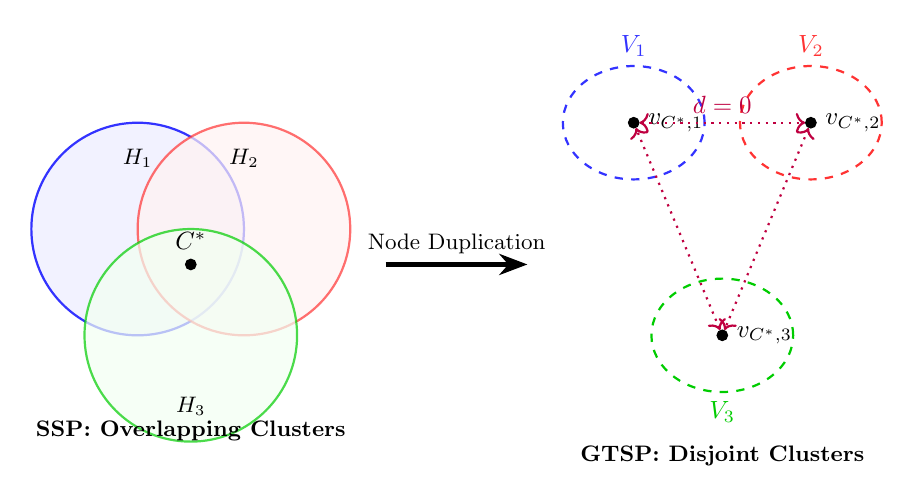
\begin{tikzpicture}[scale=0.9, every node/.style={transform shape}]
    % SSP Overlapping View (Left)
    \begin{scope}
        \draw[thick, blue!80, fill=blue!5] (0,1) circle (1.5cm);
        \draw[thick, red!80, fill=red!5, opacity=0.7] (1.5,1) circle (1.5cm);
        \draw[thick, green!80!black, fill=green!5, opacity=0.7] (0.75,-0.5) circle (1.5cm);
        
        \node at (0, 2) {\small $H_1$};
        \node at (1.5, 2) {\small $H_2$};
        \node at (0.75, -1.5) {\small $H_3$};
        
        % Intersection Node
        \node[draw, circle, fill=black, inner sep=1.5pt, label=above:{$C^*$}] (Cstar) at (0.75, 0.5) {};
        \node[below=2cm of Cstar, font=\small\bfseries] {SSP: Overlapping Clusters};
    \end{scope}

    % Reduction Arrow
    \draw[-{Stealth}, ultra thick] (3.5,0.5) -- (5.5,0.5) node[midway, above, font=\small] {Node Duplication};

    % GTSP Disjoint View (Right)
    \begin{scope}[shift={(7,0)}]
        \draw[thick, dashed, blue!80] (0,2.5) ellipse (1cm and 0.8cm) node[above=0.8cm] {$V_1$};
        \draw[thick, dashed, red!80] (2.5,2.5) ellipse (1cm and 0.8cm) node[above=0.8cm] {$V_2$};
        \draw[thick, dashed, green!80!black] (1.25,-0.5) ellipse (1cm and 0.8cm) node[below=0.8cm] {$V_3$};
        
        % Duplicated Nodes
        \node[draw, circle, fill=black, inner sep=1.5pt, label=right:{$v_{C^*,1}$}] (v1) at (0, 2.5) {};
        \node[draw, circle, fill=black, inner sep=1.5pt, label=right:{$v_{C^*,2}$}] (v2) at (2.5, 2.5) {};
        \node[draw, circle, fill=black, inner sep=1.5pt, label=right:{$v_{C^*,3}$}] (v3) at (1.25, -0.5) {};
        
        % Zero-cost "internal" edges
        \draw[<->, purple, thick, dotted] (v1) -- (v2) node[midway, above] {$d=0$};
        \draw[<->, purple, thick, dotted] (v2) -- (v3);
        \draw[<->, purple, thick, dotted] (v3) -- (v1);
        
        \node at (1.25, -2.2) {\small\bfseries GTSP: Disjoint Clusters};
    \end{scope}
\end{tikzpicture}
\caption{Complex transformation of the SSP state space into a GTSP framework. A configuration $C^*$ residing in the intersection of three clusters is duplicated into three distinct nodes, one for each cluster. The switching cost between these duplicates is zero, allowing the GTSP to effectively "pass through" multiple job requirements without cost.}
\label{fig:complex_reduction}
\end{figure}

\section{Reduction: $GTSP \rightarrow SSP$ (Reverse Equivalence)}

To complete the proof, we demonstrate that the GTSP can be viewed as a restricted instance of the SSP where tool requirements are engineered to prevent cluster overlap. 

\subsection{The Disjointness Condition}
The GTSP structure is recovered when the configuration clusters $H_j$ are naturally disjoint[cite: 43]. 

\begin{theorem}[Disjointness Condition]
If for every pair of jobs $j_k, j_j \in J$, the required tool sets satisfy $|T_k \cup T_j| > B$, then the clusters $H_k$ and $H_j$ are disjoint.
\end{theorem}

\begin{proof}
Assume for contradiction that $H_k \cap H_j \neq \emptyset$. This implies there exists at least one configuration $C$ such that $T_k \subseteq C$ and $T_j \subseteq C$. 
This requirement necessitates that $(T_k \cup T_j) \subseteq C$[cite: 222]. 
Taking the cardinality of both sides, we have $|T_k \cup T_j| \le |C|$. 
Given the magazine capacity constraint $|C| \le B$, it follows that $|T_k \cup T_j| \le B$[cite: 223]. 
This directly contradicts the initial condition $|T_k \cup T_j| > B$. 
Therefore, no such configuration $C$ exists, and $H_k \cap H_j = \emptyset$ [cite: 45-46, 224].
\end{proof}

\subsection{Equivalence of Constraints}
Under the disjointness condition, every configuration $v \in V$ belongs to exactly one cluster $H_j$. Consequently, the covering constraint $\sum_{v \in H_j} y(v) \ge 1$ from Eq. \eqref{eq:cw_cover} becomes a strict equality $\sum_{v \in H_j} y(v) = 1$ in any optimal solution[cite: 58, 226]. This matches the fundamental node-selection requirement of a GTSP tour, completing the proof of structural identity between the two problems[cite: 227].

\section{Computational Intractability and Decomposition}

The formal reduction of the Standard Tool Switching Problem (SSP) to a Generalized Traveling Salesman Problem (GTSP) reveals a state space of extreme cardinality. As established in the Colares-Wagler formulation, the number of possible magazine configurations $p = \binom{m}{B}$ grows exponentially with the total tool count $m$ and magazine capacity $B$. For industrial instances where $m=60$ and $B=20$, the vertex set $V$ contains approximately $4.19 \times 10^{15}$ configurations, rendering the construction of the full GTSP graph $(\mathcal{V}, \mathcal{E})$ computationally impossible for exact solvers.

To address this, we employ \textbf{Column Generation (CG)}, a mathematical decomposition technique that partitions the problem into a Restricted Master Problem (RMP) and a Pricing Subproblem. This approach ensures that we only evaluate a small, highly promising subset of configurations $\overline{V} \subset V$ at any given iteration.

\section{The Restricted Master Problem (RMP)}

The RMP is a linear relaxation of the non-compact formulation (Eq. 5-14), restricted to a subset of configurations $\overline{V}$ that have been previously identified as "useful".

\subsection{Formal RMP Model}
Given a subset $\overline{V}$, the RMP seeks a minimum-cost path through the known configuration nodes:
\begin{equation}
    \min z = \sum_{u \in \overline{V}} \sum_{v \in \overline{V}} d(u,v) \overline{x}(u,v)
\end{equation}
Subject to:
\begin{align}
    \sum_{v \in \overline{V} \cap H_{j}} y(v) \ge 1 & \quad \forall j \in J \quad (\text{Dual Variables: } \pi_j) \label{eq:rmp_job} \\
    \sum_{u \in \overline{V}} x(u,v) = y(v) & \quad \forall v \in \overline{V} \quad (\text{Dual Variables: } \sigma_v) \label{eq:rmp_flow}
\end{align}
Constraint \eqref{eq:rmp_job} ensures every job is covered by at least one configuration in the restricted set, while \eqref{eq:rmp_flow} maintains the sequence flow.

\subsection{Dual Variable Interpretation}
The RMP provides critical economic information via the dual variables $\pi_j$ and $\sigma_v$. The variable $\pi_j$ represents the "marginal benefit" of including a new configuration that satisfies job $j$. In the context of GTSP, these duals identify which clusters $V_j$ are currently the most "expensive" to visit, guiding the search for new nodes.

\section{The Pricing Subproblem: Generating GTSP Nodes}

The pricing step identifies a new configuration $C^* \in V \setminus \overline{V}$ that has a \textbf{negative reduced cost} $\bar{c}$. If such a configuration is found, its inclusion in the RMP is guaranteed to potentially improve the current objective value.

\subsection{Objective of the Subproblem}
The reduced cost $\bar{c}$ for a new configuration $C$ is mathematically defined as:
\begin{equation}
    \bar{c}(C) = \text{Switching Cost} - \sum_{j: T_j \subseteq C} \pi_j
\end{equation}
To minimize $\bar{c}$, the subproblem maximizes the total "bounty" collected from covered jobs minus the cost of tool swaps:
\begin{equation}
    \max \omega = \sum_{j \in J} \pi_j y(j) - \text{Transition Costs}
\end{equation}

\section{AI-Augmented Neural Pricing Oracle}

The combinatorial nature of the pricing subproblem (solving Eq. 20-22) often becomes the computational bottleneck in the CG cycle. We propose a state-of-the-art **Neural Pricing Oracle** to accelerate the discovery of optimal configurations.

\subsection{Neural Architecture: Graph Neural Networks (GNN)}
The AI agent utilizes a GNN to encode the structural relationship between tools and job requirements.
\begin{itemize}
    \item \textbf{Input:} The current dual vector $\bm{\pi}$ and the hypergraph of job requirements.
    \item \textbf{Embedding:} Tools are embedded as nodes in a graph where edges represent shared job requirements.
    \item \textbf{Output:} A probability distribution over tools, identifying the most "valuable" combination to form the next magazine configuration $C^*$.
\end{itemize}

\begin{figure}[h!]
\centering
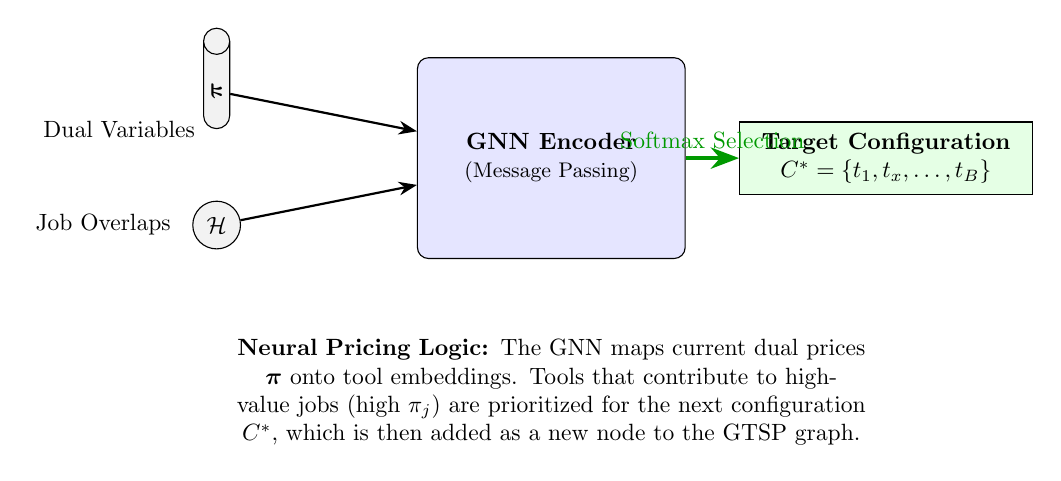
\begin{tikzpicture}[scale=0.85, every node/.style={transform shape}]
    % Central Neural Block
    \node[draw, rectangle, fill=blue!10, minimum width=4cm, minimum height=3cm, rounded corners] (GNN) at (0,0) {
        \begin{tabular}{c} \textbf{GNN Encoder} \\ \small (Message Passing) \end{tabular}
    };

    % Inputs
    \node[draw, cylinder, rotate=90, fill=gray!10, minimum height=1.5cm] (Duals) at (-5, 1) {$\bm{\pi}$};
    \node[draw, circle, fill=gray!10] (Graph) at (-5, -1) {$\mathcal{H}$};
    \node[left=0.2cm of Duals] {Dual Variables};
    \node[left=0.2cm of Graph] {Job Overlaps};

    % Arrows to GNN
    \draw[-{Stealth}, thick] (Duals) -- (GNN);
    \draw[-{Stealth}, thick] (Graph) -- (GNN);

    % Outputs
    \node[draw, rectangle, fill=green!10, minimum width=3cm] (Config) at (5,0) {
        \begin{tabular}{c} \textbf{Target Configuration} \\ $C^* = \{t_1, t_x, \dots, t_B\}$ \end{tabular}
    };
    \draw[-{Stealth}, ultra thick, green!60!black] (GNN) -- (Config) node[midway, above] {Softmax Selection};

    % Caption-like node
    \node[text width=12cm, align=center] at (0, -3.5) {
        \textbf{Neural Pricing Logic:} The GNN maps current dual prices $\bm{\pi}$ onto tool embeddings. Tools that contribute to high-value jobs (high $\pi_j$) are prioritized for the next configuration $C^*$, which is then added as a new node to the GTSP graph.
    };
\end{tikzpicture}
\caption{Architectural overview of the AI Pricing Agent within the Column Generation framework.}
\label{fig:neural_cg}
\end{figure}

\subsection{Optimality Guarantees}
While the AI agent provides rapid heuristic candidates, the system remains an \textbf{exact solver}. If the AI-generated $C^*$ has $\bar{c} < 0$, it is added to the RMP. If the AI agent fails to find such a column, an exact MILP pricing solver is invoked. This "Neural-Exact Hybrid" ensures that the speed of ML is harnessed without sacrificing the mathematical guarantee of the global optimum.

\section{Conclusion}
This report has formally defined the Tool Switching Problem (SSP) through the non-compact formulation of \textcite{Colares2026} and established its mathematical equivalence to the Generalized Traveling Salesman Problem (GTSP). By duplicating configuration vertices to resolve the "Overlap Problem," we have mapped the SSP into a disjoint GTSP state space. Given the exponential number of configurations, the Column Generation framework serves as the primary computational engine, further enhanced by AI-driven pricing strategies that utilize the structural dependencies of shared tools. This hybrid approach represents the current state-of-the-art in solving large-scale combinatorial manufacturing problems.

\newpage
\printbibliography

\end{document}